\documentclass[letterpaper]{article} % DO NOT CHANGE THIS
% NeusymBridge uses double-blind review: keep the [submission] option (AAAI-27 Author Kit).
\usepackage[submission]{aaai2027}  % DO NOT CHANGE THIS
\usepackage[hyphens]{url}  % DO NOT CHANGE THIS
\usepackage{graphicx} % DO NOT CHANGE THIS
\urlstyle{rm} % DO NOT CHANGE THIS
\def\UrlFont{\rm}  % DO NOT CHANGE THIS
\usepackage{natbib}  % DO NOT CHANGE THIS AND DO NOT ADD ANY OPTIONS TO IT
\usepackage{caption} % DO NOT CHANGE THIS AND DO NOT ADD ANY OPTIONS TO IT
\frenchspacing  % DO NOT CHANGE THIS
\usepackage{booktabs}
\usepackage{amsmath}
\usepackage{multirow}
\usepackage{array}
\newcommand{\clade}{\textsc{Clade}}
\pdfinfo{
/TemplateVersion (2027.1)
}
\setcounter{secnumdepth}{2}

\title{\clade{}: Category-Level Answering from Deficient Evidence\\in Retrieval-Augmented Language Models}
\author{Anonymous Submission}
\affiliations{}

\begin{document}

\maketitle

\begin{abstract}
Retrieval-augmented systems often hand a model a page that is true and
relevant but names only the family of the answer: the question asks which
disease a drug treats, and the page says ``hyperlipidemia'' where the answer is
``familial hyperlipidemia.'' Work on sufficient context treats such pages as
simply insufficient. We argue they form a distinct case, \emph{resolvable
insufficiency}: the text cannot settle the answer, but its family name indexes
a short candidate list in an ontology. Models meet it with \clade{}
(category-level answering from deficient evidence): they answer instead of
declining or looking further. On 856 PrimeKG questions, a family-only page
weakens the push toward ``not enough information'' by 13.8 points relative to a
silent page (pooled over three 7--8B models, $p = 4\times10^{-5}$; significant
for two of the three individually), and the freed answers are about as often
wrong as right. A counterfactual edit isolates the cause: replacing the disease
name with its family name lowers declines by 17.4 points relative to deleting
the sentence. Confidence (AUROC 0.59--0.72 on family-only pages, against
0.73--0.87 on named pages), a 14B model (58\% precision, against 96\%) and an
instruction to decline (more declines on every kind of page) all leave \clade{}
in place. It replicates on species interactions from GloBI, with a taxonomy as
the symbolic structure (900 questions; decline effect $-14.3$ points,
$p = 10^{-9}$), where the freed answers are mostly wrong. Resolving the
insufficiency is only partly solved: the ontology list holds the answer 98.5\%
of the time once the family is known, but the family is found from the page
only 19.8\% of the time, and a popularity prior beats both the model and
literature evidence at choosing within it. The results locate where a neural
reader should hand over to symbolic knowledge, and which steps of that handover
remain open.
\end{abstract}

\section{Introduction}

\begin{figure*}[t]
\centering
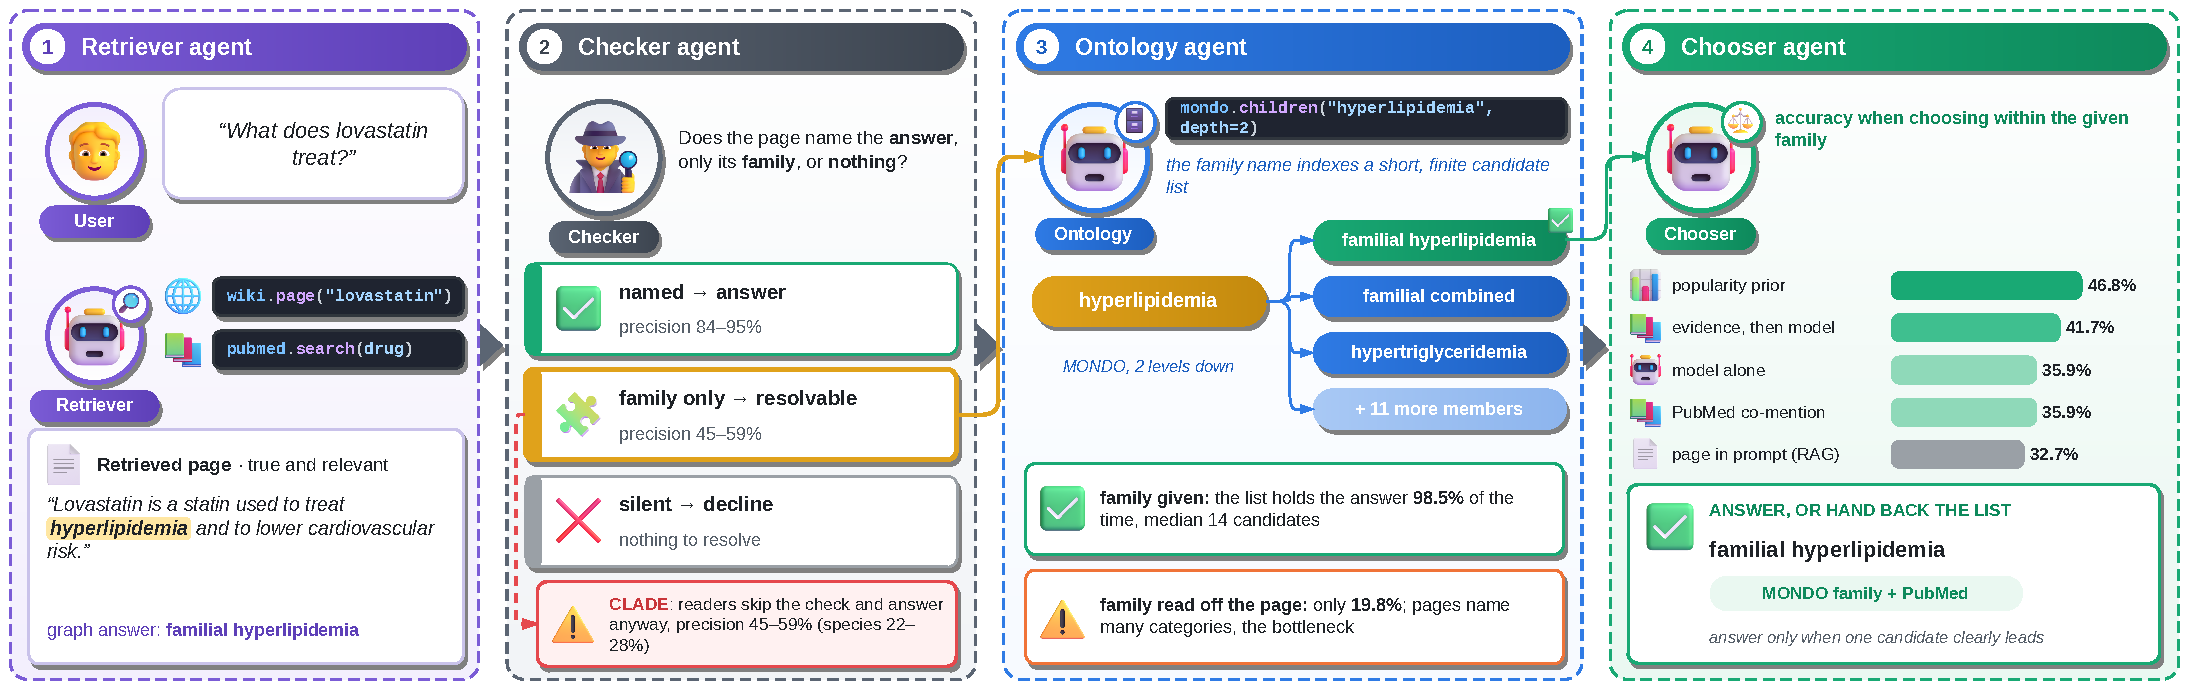
\includegraphics[width=\textwidth]{fig_concept.pdf}
\caption{Resolvable insufficiency, drawn as a proposed agent workflow with the
bottleneck we measure at each step. The dashed red path is \clade{}: the reader
answers from the family-only page instead of handing it on. The retrieved page is true and relevant but
names only the answer's family. A page-type check should route it away from
answering; an ontology step turns the family name into a short candidate list;
a chooser picks from it or hands the list back. Only the ontology step works
reliably today.}
\label{fig:concept}
\end{figure*}

A retrieval-augmented system answers a question by reading a page
\citep{lewis2020rag}. Much recent work asks what the model should do when the
page is not enough. The usual framing is binary: the context is sufficient or
it is not \citep{joren2025sufficient}, and a well-behaved model answers in the
first case and abstains in the second \citep{wen2025abstention}.

Many pages fall between these cases in a structured way. Consider the question
``What does lovastatin treat?'' with the answer \emph{familial
hyperlipidemia}, and a page that says ``lovastatin is used to treat
hyperlipidemia'' (Figure~\ref{fig:concept}). The page is true and relevant. It
rules out every disease that is not a hyperlipidemia. It does not say which
one. A model can answer anyway, say ``not enough information,'' or look
further. Looking further has a natural symbolic form: a disease ontology lists
the members of the family, and each can be checked.

We call this case \emph{resolvable insufficiency}. The page is insufficient,
because it cannot settle the answer. It is resolvable in the sense of candidate-space reduction: the family name
it does contain indexes a short, finite candidate set in a knowledge
structure. Whether a system can then pick the right member is a separate
question, which we also measure. When a model answers from such a page anyway,
we call the behavior \clade{}: category-level answering from deficient
evidence. This is the point where a neural reader and a symbolic resource
have the most to offer each other, and it is common: in our data, text names
the exact disease for only a minority of graph facts, and part of the rest is
written at the family level.

We ask three questions. How much of a biomedical knowledge graph does text
name, and does a family name help a model at all? When a page names only the
family, does a model stop declining, and are the answers it gives instead
right? And can an ontology turn the family name back into the answer?

Our contributions are:
\begin{itemize}
\item We define resolvable insufficiency and the failure it invites, \clade{},
and measure it per fact, by
classifying each page as naming the answer, naming only its family in the
MONDO disease ontology, or naming nothing.
\item We show that, pooled over three 7--8B models from different families, a
family-only page weakens abstention relative to a silent page, using a design
that compares each question with itself with and without the page, and that
the answers it frees are about as often wrong as right, far less reliable than
answers from a page that names the disease.
\item We isolate the cause with a counterfactual edit of the same pages, show
that confidence thresholds, a larger model and an instruction to decline do not
remove the effect, and replicate it on species interactions with a taxonomy.
\item We decompose ontology-based recovery into finding the family, listing
its members, and choosing among them, and show that the first step is the
bottleneck, while a popularity prior is a strong baseline for the last.
\end{itemize}

\section{Related Work}

\paragraph{Insufficient context in RAG.}
Retrieval failures are a recognized failure point of RAG systems
\citep{barnett2024seven}. \citet{joren2025sufficient} introduce sufficient
context as a lens on RAG errors, label contexts as sufficient or insufficient,
and show that models often answer correctly even from insufficient context and
hallucinate rather than abstain. They note that a context can narrow the answer
without settling it, but treat it as insufficient. Models are also known to be
distracted by irrelevant context \citep{shi2023distracted,yoran2024robust}, and
\citet{setiawan2026misleading} show that misleading passages collapse
prompt-based abstention while missing passages do not. Our case differs from
both: the page is neither irrelevant nor misleading. It is correct and points
in the right direction, and we show that this alone is enough to weaken
abstention.

\paragraph{Partial support and selective answering.}
Self-RAG \citep{asai2024selfrag} trains a model to judge whether a passage
fully or partially supports its output, and ALCE \citep{gao2023alce} grades
citations by whether they support a claim. CRAG \citep{yan2024crag} scores
retrieved documents and searches again when they are weak, and SURE-RAG
\citep{qiu2026sure} verifies whether evidence is sufficient before answering.
These methods recognize partial support, but not what kind of information is
missing. A family name is a specific, structured kind of partial evidence:
it says exactly which step is missing and where to look for it.

\paragraph{Abstention.}
Surveys and benchmarks document that models often answer when they should
not \citep{wen2025abstention,kirichenko2025abstentionbench}, including in
medicine \citep{machcha2026abstain}, and propose methods to detect knowledge
gaps \citep{feng2024abstain,kadavath2022know}. These works measure whether a
model declines. We measure which kind of evidence makes it stop declining.

\paragraph{Ontologies and taxonomies in retrieval.}
OG-RAG \citep{sharma2024ograg} grounds retrieval in a domain ontology, and
TaSR-RAG \citep{sun2026tasr} uses a taxonomy to structure multi-hop retrieval.
The broader program of combining language models with knowledge graphs is
surveyed by \citet{pan2024unifying}, and neuro-symbolic AI more generally by
\citet{garcez2023third}. These methods use symbolic structure for every query.
We study the specific condition under which the page itself signals that a
symbolic step is needed, and measure how far that step gets.

\paragraph{What text contains.}
\citet{mallen2023trust} and \citet{kandpal2023longtail} relate model knowledge
to entity popularity and to the number of relevant pretraining documents, and
LMEnt \citep{gottesman2026lment} traces entity mentions through a pretraining
corpus. These studies work at the level of entities. We measure, for each fact,
at what level of specificity the text names it.

\section{Setting and Data}

\paragraph{Facts and ontology.}
We use drug--disease edges from PrimeKG \citep{chandak2023primekg}, whose
indication and contraindication relations come from DrugCentral. Diseases are
identified by MONDO \citep{vasilevsky2022mondo}, which we rebuild as a directed
child-to-parent table of 17,801 edges over 11,788 diseases; 3,182 parent terms
have two or more children.

\paragraph{Text.}
For each drug we use its English Wikipedia article and a set of PubMed
abstracts retrieved per drug with a separate query budget for each relation.
Wikipedia markup is cleaned before use: templates, tables, reference tags and
file links are removed, and links are reduced to their visible text.

\paragraph{How a page names a fact.}
For each edge we classify the drug's text into one of three groups.
\emph{Named}: the text contains the disease's exact name or an alternative
name taken from Wikipedia redirects to the disease's article, which include
synonyms, lay terms and abbreviations. \emph{Family-only}: the text contains
none of these but names one of the disease's MONDO ancestors within two
levels. \emph{Silent}: the text names neither. To separate
real mentions from coincidence, each edge is paired with three diseases the
drug has no relation to, and the same matcher is run on them.

\section{How Much Does Text Reach?}

We first measure, on 1,800 PrimeKG edges (600 per relation for indication,
contraindication and off-label use), how often the drug's Wikipedia article
names the disease and how often a model knows the fact closed book. The model
picks the true disease from five options by mean token log-probability.

\begin{table}[t]
\centering
\small
\begin{tabular}{lcc}
\toprule
 & Model knows it & Model does not \\
\midrule
Text names it & 5.2 & 6.2 \\
Text does not & 22.2 & 66.4 \\
\bottomrule
\end{tabular}
\caption{Share of 1,800 PrimeKG facts (\%) by whether Wikipedia names the
disease and whether Qwen2.5 0.5B picks it from five options closed book.}
\label{tab:boxes}
\end{table}

Table~\ref{tab:boxes} crosses the two; here ``names it'' means the exact or an
alternative name, so facts named only by their family count as not named. For
two thirds of the facts, the text does not name the disease and the model does
not know the answer. The ``knows it anyway'' cell is mostly chance: accuracy on
facts the text does not name is 25.1\% against a 20\% chance rate, about 6\%
above chance after correction. A second corpus helps little: on a separate
sample measured in both corpora, the share not named is 84.9\% in Wikipedia,
81.1\% in PubMed abstracts and 77.5\% in both.

\paragraph{A family name alone does not help the model.}
If a family name carried useful signal, facts whose text names only the family
would be easier for the model than facts whose text is silent. Testing this
inside each relation and pooling with relation as a stratum on Qwen2.5 7B,
family-only facts differ sharply from named facts (Mantel--Haenszel odds ratio
0.27, 95\% CI 0.17--0.43, $p = 9\times10^{-9}$) and not measurably from
silent facts (odds ratio 1.10, 95\% CI 0.80--1.53, $p = 0.61$). The cleanest
case is indications at 7B: 44.68\% correct for family-only facts against
43.95\% for silent facts. For contraindications the figures are 18.75\% and
23.35\%. An exact name raises the odds that the model knows a fact about
3.7-fold; a family name gives no measurable help on its own.

This motivates the rest of the paper. The family name is the most common form
of partial evidence in this data, and the model cannot use it by itself. The
question is what happens when such a page is placed in front of the model at
answer time, and whether a symbolic step can make use of it.

\section{\clade{}: Abstention Under Family-Only Evidence}

\subsection{Design}

\paragraph{Questions.}
We build 856 multiple-choice questions from indication and contraindication
edges: 300 whose page names the answer, 256 whose page names only its family,
and 300 whose page is silent (150 per relation and group, except 106 family-only
contraindications, the most available). Each question offers five diseases and
a sixth option, ``Not enough information to tell,'' labeled A to F. Wrong
options come from the answer's MONDO neighborhood: its siblings first, then its
cousins (the other grandchildren of its grandparent), and random diseases only
when those run out. Neighbors exclude the answer's own ancestors and
descendants and any other disease the drug is related to by the same
relation. Most wrong options thus share the answer's family, so a family name
eliminates few of them.

\paragraph{Pages.}
Each question is asked twice: once closed book and once with a passage from
the drug's text, its cleaned Wikipedia article followed by its PubMed
abstracts. The passage is the first 800 characters of that text plus a
280-character window on each side of every mention of the disease or its
family, merged where windows overlap and capped at 1,800 characters; for
silent questions it is therefore the opening of the text. Edges whose cleaned
passage no longer shows the
answer or family are replaced by other edges.

\paragraph{Implementation.}
All models run on CPU with Hugging Face Transformers. Prompts are scored in
batches with left padding and explicit position indices. For the recovery
experiment, the prompt prefix shared by all candidates is encoded once and
reused; a sample of these scores is checked against a full forward pass
before each run. Code and data splits will be released.

\paragraph{Models and scoring.}
We test five instruction-tuned models: Qwen2.5 0.5B, 7B and 14B
\citep{qwen2025qwen25}, OLMo~2 7B \citep{olmo2024olmo2}, and Granite~3.1 8B
\citep{granite2024}. The prompt lists the options, and the model's answer is
the option letter with the highest next-token probability, renormalized over
the six letters. A question is \emph{declined} when the model picks ``Not
enough information.''

\paragraph{Controls.}
Two differences between the groups could produce a gap on their own. First,
family-only questions more often have all four distractors from the
neighborhood, which are harder to eliminate. We therefore analyze only such
questions (106 named, 215 family-only and 160 silent).
Second, the groups contain different facts, and some facts are harder than
others even without a page. We therefore compare, for each question, its
outcome with the page against its outcome closed book, and then compare this
page effect between family-only and silent questions. The difference of these
page effects is our main measure. Confidence intervals come from 5,000
bootstrap resamples of questions. To pool across the three 7--8B models, we
average each question's page effect over the models before comparing groups,
so each question counts once. The supplementary material gives the passage
and prompt formats, sampling details, formulas, queries and full result
tables.

\subsection{Results}

\begin{table}[t]
\centering
\small
\setlength{\tabcolsep}{3.2pt}
\begin{tabular}{llcccc}
\toprule
Model & Page & Correct & Wrong & Declines & Prec. \\
\midrule
\multirow{3}{*}{Qwen2.5 7B} & named & 71.7 & 3.8 & 24.5 & 95.0 \\
 & family & 26.5 & 18.1 & 55.3 & 59.4 \\
 & silent & 13.8 & 2.5 & 83.8 & 84.6 \\
\midrule
\multirow{3}{*}{OLMo 2 7B} & named & 77.4 & 15.1 & 7.5 & 83.7 \\
 & family & 37.2 & 44.7 & 18.1 & 45.5 \\
 & silent & 30.6 & 24.4 & 45.0 & 55.7 \\
\midrule
\multirow{3}{*}{Granite 3.1 8B} & named & 72.6 & 7.5 & 19.8 & 90.6 \\
 & family & 30.2 & 26.5 & 43.3 & 53.3 \\
 & silent & 15.0 & 10.0 & 75.0 & 60.0 \\
\midrule
\multirow{3}{*}{Qwen2.5 0.5B} & named & 77.4 & 14.2 & 8.5 & 84.5 \\
 & family & 34.4 & 55.8 & 9.8 & 38.1 \\
 & silent & 28.7 & 50.6 & 20.6 & 36.2 \\
\midrule
\multirow{3}{*}{Qwen2.5 14B} & named & 67.9 & 2.8 & 29.2 & 96.0 \\
 & family & 24.2 & 17.2 & 58.6 & 58.4 \\
 & silent & 11.9 & 2.5 & 85.6 & 82.6 \\
\bottomrule
\end{tabular}
\caption{Outcomes with the page (\%), questions whose four distractors all come from the answer's neighborhood
(106 named, 215 family-only, 160 silent). Precision is the share correct among
questions the model answered.}
\label{tab:outcomes}
\end{table}

\begin{figure*}[t]
\centering
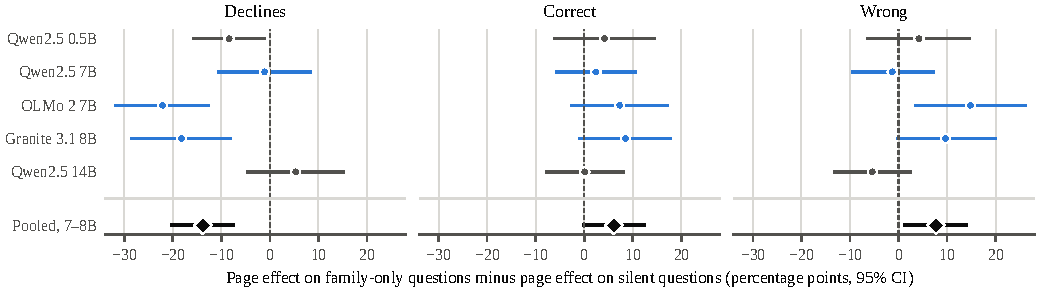
\includegraphics[width=\textwidth]{fig_forest.pdf}
\caption{What a family-only page does, relative to a silent page. For each
question, the page effect is its outcome with the page minus its outcome
closed book; the plot shows the mean page effect on family-only questions
minus that on silent questions, with 95\% bootstrap intervals. The pooled row
averages each question over the three 7--8B models (481 questions). Gray rows
are outside the pooled set.}
\label{fig:forest}
\end{figure*}

\paragraph{With the page in hand, models decline less when it names only the
family.}
Table~\ref{tab:outcomes} gives outcomes with the page. In all three 7--8B
models, a family-only page leads to fewer declines than a silent page: 55.3\%
against 83.8\% for Qwen2.5 7B, 18.1\% against 45.0\% for OLMo~2, and 43.3\%
against 75.0\% for Granite. The model answers more, and it answers less
precisely: among answered questions, family-only pages give 45.5--59.4\%
precision, against 83.7--95.0\% for pages that name the disease.


\paragraph{The effect is the page's, not the questions'.}
The raw comparison also reflects differences between the facts in each group.
With no page, family-only questions already produce more wrong answers than
silent ones in all three models (32.6\% against 15.6\% for Qwen2.5 7B, 56.7\%
against 51.2\% for OLMo~2, 33.0\% against 26.2\% for Granite; supplement), so part of the gap in Table~\ref{tab:outcomes} comes from which facts
fall in which group. Figure~\ref{fig:forest} removes this by comparing each
question with itself. Pooled over the three
7--8B models, a page raises declines by 14.7 points on family-only questions
and by 28.5 points on silent ones, a difference of 13.8 points (95\% CI
$-20.3$ to $-7.5$, $p = 3.6\times10^{-5}$), which holds after a Bonferroni
correction for the three outcomes ($p = 1.1\times10^{-4}$). The freed
answers split about evenly. A page lowers wrong answers by 11.0 points on
family-only questions and by 18.8 on silent ones, a difference of 7.7 points
(95\% CI 1.2 to 14.0, $p = 0.019$; 0.056 after correction), and it lowers
correct answers by 3.7 and 9.8 points, a difference of 6.1 points (95\% CI
$-0.1$ to 12.4, $p = 0.058$). The decline effect is individually significant
for OLMo~2 ($-22.1$ points, $p = 6\times10^{-6}$) and Granite ($-18.2$ points,
$p = 0.0006$). Qwen2.5 7B shows no difference in its page effect ($-1.1$
points, $p = 0.82$): it already declines family-only questions less often
without a page (32.1\% against 59.4\%), and the page
raises declines by the same amount in both groups.

\paragraph{Robustness.}
The raw pattern holds for both relations in all three models (per-relation
rates in the supplement), and the 0.5B model shows the decline effect as well
($-8.4$ points, 95\% CI $-15.7$ to $-1.1$, $p = 0.027$).

The decline effect depends on how large the named family is. Splitting the
family-only questions into thirds by the number of members, the pooled effect is
$-17.3$ points (95\% CI $-26.2$ to $-8.2$) for families of up to 10 members
and $-18.4$ ($-26.6$ to $-10.3$) for 11--20 members, but only $-6.5$
($-15.7$ to $+3.0$) for larger families (Figure~\ref{fig:fixes}c). A narrow
family makes the page look answerable.

\subsection{The Family Name Causes \clade{}}

\begin{figure}[t]
\centering
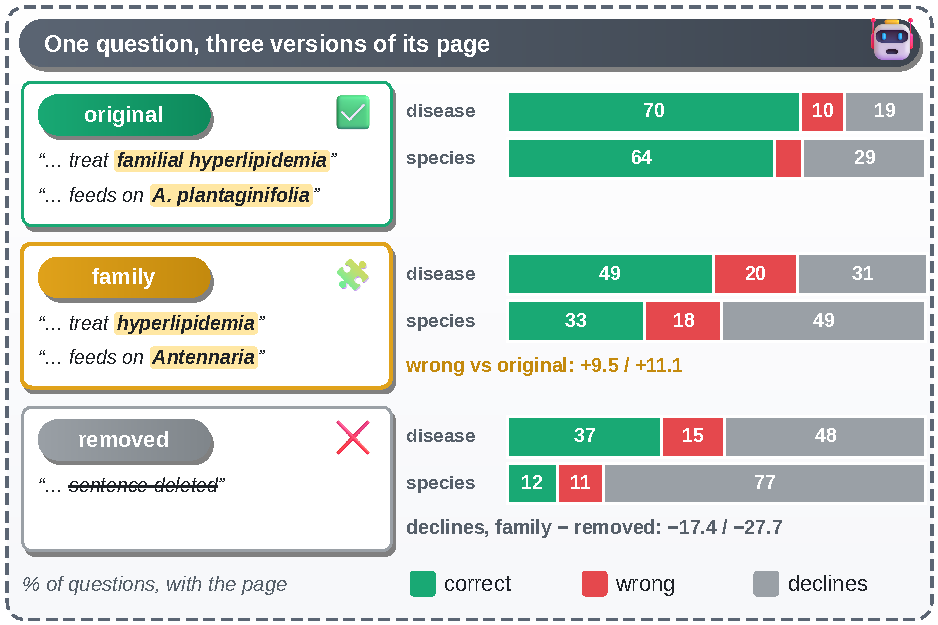
\includegraphics[width=\columnwidth]{fig_edit.pdf}
\caption{Counterfactual page edit on the same named questions, for diseases
(PrimeKG, 130 questions) and species (GloBI, 255). \emph{Family} replaces every
mention of the answer with its parent; \emph{removed} deletes the sentences
that mention it. Outcomes with the page (\%), averaged over three 7--8B
models.}
\label{fig:edit}
\end{figure}

The comparison above is between different facts. To hold the fact fixed, we
edit the page itself. For the 130 named questions whose answer has a parent in
MONDO, we build two versions of each page: \emph{family} replaces every mention
of the answer with its parent's name, and \emph{removed} deletes the sentences
that mention it. Question, options and model are unchanged; only the page
differs.

Figure~\ref{fig:edit} shows the result. Relative to the original page, the
family version lowers correct answers by 21.0 points (95\% CI $-26.9$ to
$-15.6$) and raises wrong answers by 9.5 (5.9 to 13.6), while declines rise by
only 11.5 (7.4 to 15.9). Relative to deleting the mention, keeping the family
name lowers declines by 17.4 points ($-23.6$ to $-11.5$) and raises both wrong
answers, by 5.1 points (0.5 to 10.3), and correct ones, by 12.3 (6.9 to
17.9). Each model shows the same order: Qwen2.5 7B declines 70.0\% of the
removed versions and 43.8\% of the family versions, Granite 56.2\% and
40.8\%, OLMo~2 18.5\% and 7.7\%. The family name therefore produces both
effects seen in the observational comparison: it suppresses declining, and the
answers it frees split between right and wrong.

\subsection{Three Easy Fixes Leave \clade{} in Place}

\begin{figure*}[t]
\centering
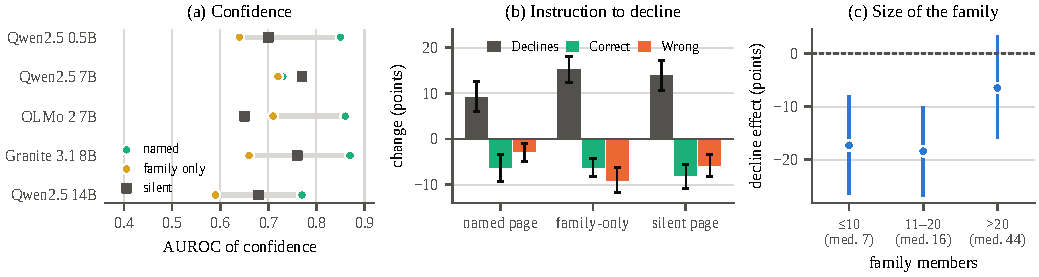
\includegraphics[width=\textwidth]{fig_fixes.pdf}
\caption{Three easy fixes. (a) Confidence separates right from wrong answers
less well on family-only pages in every model. (b) An instruction to decline
when the page names only a broad category raises declines on every kind of page
(pooled over three 7--8B models, 95\% CIs). (c) The decline effect of a
family-only page is concentrated in small and medium families.}
\label{fig:fixes}
\end{figure*}


\paragraph{Confidence does not flag these answers.}
A system could answer only when the model is confident. Figure~\ref{fig:fixes}a
shows that confidence separates right from wrong answers less well on
family-only pages than on named pages in every model (AUROC 0.59--0.72 against
0.73--0.87). The wrong answers are confident: the mean probability of a wrong
choice on a family-only page is 0.77--0.99 for the 7B and larger models, and
0.99 for Qwen2.5 14B. A threshold that keeps most correct answers keeps most of
these wrong ones too.

\paragraph{Scale does not remove the gap.}
Qwen2.5 14B is more precise on named pages than any smaller model (96.0\%,
Table~\ref{tab:outcomes}), but on family-only pages its precision stays at
58.4\%, and it gives 14.7 more points of wrong answers on family-only pages than
on silent ones ($p = 6\times10^{-6}$). Like Qwen2.5 7B, it already declines
family-only questions less often without a page, and its page effect does not
differ between the groups ($+5.3$ points, $p = 0.29$).


\paragraph{An instruction to decline is not targeted.}
The simplest remedy is to tell the model: if the page names only a broad
category that contains the answer, choose ``Not enough information.''
Figure~\ref{fig:fixes}b shows that the instruction raises declines on
family-only pages by 15.2 points (95\% CI 12.4 to 18.1), but also by 14.0 on silent pages and by 9.1
on pages that name the answer, where it costs 6.3 points of correct answers
($-9.4$ to $-3.5$).
Precision on family-only pages stays at 47.9--64.9\% after the instruction,
far below the 89.6--94.7\% the same prompt gives on named pages (per-model
rates in the supplement). The instruction does not help because the models do
not tell a family name from an answer.

\paragraph{What the result means.}
A silent page pushes a model toward ``not enough information''; a page naming
only the family pushes it much less, because it is relevant. The answers this
frees are about as often wrong as right: the family name lets the model guess
within a smaller space without telling it which member is meant, and a system
that treats a relevant page as permission to answer will do so at 45--59\%
precision while citing a relevant source.

\subsection{\clade{} in a Second Domain: Species Interactions}

\begin{table}[t]
\centering
\footnotesize
\setlength{\tabcolsep}{3pt}
\begin{tabular}{lrr}
\toprule
 & PrimeKG & GloBI \\
\midrule
Questions, pooled (all-sibling) & 481 & 833 \\
Decline effect, family $-$ silent & $-13.8$ & $-14.3$ \\
Wrong effect, family $-$ silent & $+7.7$ & $+11.6$ \\
Precision, named page (\%) & 84--95 & 84--95 \\
Precision, family-only page (\%) & 45--59 & 22--28 \\
AUROC, named page & .73--.87 & .82--.86 \\
AUROC, family-only page & .66--.72 & .52--.68 \\
Edit: declines, family $-$ removed & $-17.4$ & $-27.7$ \\
Edit: wrong, family $-$ removed & $+5.1$ & $+6.7$ \\
Edit: correct, family $-$ original & $-21.0$ & $-30.8$ \\
\bottomrule
\end{tabular}
\caption{The same tests on drug--disease facts (PrimeKG, MONDO) and on
species interactions (GloBI, taxonomy), for the three 7--8B models. Effects
in points; ranges are over models. All effects shown have 95\% CIs that
exclude zero.}
\label{tab:globi}
\end{table}

To test whether the effect depends on medicine or on MONDO, we repeat the
abstention test and the counterfactual edit on species interactions from
GloBI \citep{poelen2014globi}. We keep four relations (\emph{eats},
\emph{preys on}, \emph{parasite of}, \emph{pollinates}) between species,
use the consumer's Wikipedia article as the page, and use GloBI's taxonomy
(species, genus, family) in place of MONDO. A page is named if it gives the
partner's binomial, its abbreviated form or a common name from Wikipedia
redirects, and family-only if it gives only the genus or family. Wrong options
are species of the same genus, then of the same family, and never a recorded
partner. The question set has 75 questions per group and relation (900 in all).

Exact partners are rarely written down: of 23,694 measured edges, the page
names the partner species for 3.9\% and only its genus or family for 7.1\%.
Table~\ref{tab:globi} shows that every result carries over. A page raises
declines by 12.1 points on silent questions but lowers them by 2.3 on
family-only ones, a difference of $-14.3$ points ($p = 1.4\times10^{-9}$);
the freed answers are mostly wrong ($+11.6$ points, $p = 2.5\times10^{-8}$;
correct $+2.7$, $p = 0.09$). Family-only precision falls to 22--28\%, since
species of one genus are harder to tell apart than diseases of one family. The
counterfactual edit is stronger than on PrimeKG: keeping the genus name instead
of deleting the sentence lowers declines by 27.7 points ($-32.2$ to $-23.5$)
and raises wrong answers by 6.7 (3.4 to 10.2; Figure~\ref{fig:edit}). Resolvable insufficiency is a
property of how text names facts that sit in a hierarchy, not of one domain.

\section{Resolving the Insufficiency with an Ontology}

If a family name is the most common form of partial evidence, an ontology
should be able to use it. We decompose this into three steps: identify the
family from the page, list its members, and choose among them.

\subsection{Design}

We use the 410 indication and contraindication edges whose text names only
the family, in Wikipedia and PubMed together. A pick counts as correct when it
is any disease the drug has the same relation to, since a family list holds
2.47 true answers on average and over half hold more than one.

\paragraph{Listing the members.}
The \emph{given-family} list takes the narrowest ancestor of the answer that
the text names and lists its MONDO descendants up to two levels below it,
capped at 64. It assumes the right family is known. The \emph{page-built} list
instead finds every MONDO category with at least two children whose name
appears in the drug's Wikipedia article, and takes the union of their
descendants. A list larger than 64 candidates counts as too broad.

\paragraph{Choosing a member.}
We compare Qwen2.5 7B choosing from the given-family list without the page
and with it; Wikipedia evidence (the candidate's own article names the drug);
PubMed evidence (the number of abstracts naming both the drug and the
candidate, with a relation-specific qualifier); PubMed evidence normalized by
the candidate's total number of abstracts; and a popularity prior, the
candidate with the most PubMed abstracts regardless of the drug. Two baselines
use no ontology: a list of the same size with the answer and random diseases,
and the same list with the page in the prompt, which is what a standard RAG
system sees. Paired comparisons use McNemar's test \citep{mcnemar1947}.

\subsection{Results}

\begin{figure}[t]
\centering
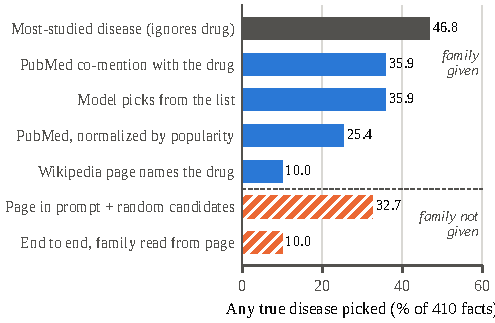
\includegraphics[width=\columnwidth]{fig_recovery.pdf}
\caption{Recovery on 410 family-only facts. Blue and gray bars choose within
the given family; hatched bars do not receive the family.}
\label{fig:recovery}
\end{figure}

\begin{table}[t]
\centering
\small
\setlength{\tabcolsep}{4pt}
\begin{tabular}{lcc}
\toprule
 & Given family & Page-built \\
\midrule
Usable lists (of 410) & 410 & 166 \\
List contains the sampled answer & 98.5\% & 19.8\% \\
List contains any true answer & 99.5\% & 24.6\% \\
Median list size & 14 & 32 \\
\bottomrule
\end{tabular}
\caption{Candidate lists. Coverage is over all 410 facts; of the 244 unusable
page-built lists, 209 exceed 64 candidates and 35 have no usable category.}
\label{tab:lists}
\end{table}

\paragraph{Given the family, the ontology narrows the search well.}
Table~\ref{tab:lists} shows that when the right family is known, its member
list contains the answer 98.5\% of the time with a median of 14 candidates.
List coverage is not accuracy, however: a member still has to be chosen.

\paragraph{Finding the family is the bottleneck.}
When the list is built from the categories the page actually names, it
contains the answer for only 19.8\% of facts. A page names a median of five
categories, and for 209 of 410 facts their union exceeds 64 candidates. The
page does name the right family, but it also names others, and nothing in the
text marks which one belongs to the answer. Reading more text makes this worse,
not better. Building the list from the Wikipedia article and the PubMed
abstracts together raises the median number of categories named to 17; 391 of
410 lists then exceed 64 candidates, and only 3.7\% of facts get a usable list
that contains the answer. The bottleneck is not missing text but too many
candidate families.

\paragraph{Within a family, popularity beats evidence.}
Figure~\ref{fig:recovery} compares ways of choosing. Given the family, the
model alone is right 35.9\% of the time, and 32.4\% when it also sees the
page. PubMed co-mention also reaches 35.9\%, and taking evidence first
(Wikipedia and PubMed combined) and the model's pick otherwise reaches 41.7\%,
which beats the model alone (59 against 35 discordant facts, $p = 0.018$). The
popularity prior, which ignores the drug, reaches 46.8\%, the highest of all.
Once co-mention counts are divided by the candidate's total abstracts, they
fall to 25.4\%, so the drug-specific part of the literature signal is weak.
Wikipedia rarely helps, because a candidate's article names the drug in only
3.9\% of cases. The two baselines without an ontology reach 34.9\% (random
list) and 32.7\% (page in prompt). Their lists exclude the drug's other true
partners, so under any-true-answer scoring they are not at matched chance with
the family lists and serve as reference points only.


\paragraph{What the misses look like.}
Some misses choose a better-studied member of the family (for carboplatin,
ovarian carcinoma rather than the rarer germ cell tumor the graph records), and
some are true facts the graph does not list (moxifloxacin for Legionnaires'
disease), so evaluation against a graph understates recovery for every method
alike. The supplement lists examples.

\paragraph{End to end.}
Without being given the family, building the list from the page and choosing
by evidence recovers the answer for 10.0\% of facts. The page-in-prompt
baseline reaches 32.7\%, helped by a family name that lets it eliminate
random distractors outside the family. With lists built from both corpora,
end-to-end recovery falls to 1.5\%, for the reason given above.

\section{Discussion}

\paragraph{Where the neural reader should hand over.}
The results give a precise handover point. Under resolvable insufficiency, a
model reading a family-only page shows \clade{}: it treats the page as license
to answer, with markedly lower precision than on named
facts. A symbolic structure can turn the same family name into a short
list that almost always contains the answer, but only if the right family is
identified. A neuro-symbolic system should therefore do three things the
models do not: recognize that a page names a family rather than the answer,
identify which family belongs to the question, and choose within it with a
baseline that is at least as strong as popularity.

\paragraph{A procedure that follows from the results.}
The findings suggest a simple decision procedure for a retrieval-augmented
system facing a page about the question's subject.
\begin{enumerate}
\item Check whether the page names the answer type at the required level.
If it does, answer from the page.
\item If the page names only categories, identify which category belongs to
the question. If none can be identified, decline.
\item List the category's members from the ontology and score them with
evidence and with a popularity prior; answer only if a candidate clearly
leads, and otherwise return the short list or decline.
\end{enumerate}
The models we tested skip the first two checks, which is \clade{}: a relevant
page is treated as permission to answer, and neither confidence nor an instruction recovers
step 1. Step 2 is the weakest link in our measurements and the
most promising target for a learned component. For step 3, any system should
report a popularity prior: in our data it beats the model, literature counts
and a standard RAG baseline.

\paragraph{Partial evidence has a type.}
Sufficient-context methods ask whether a page settles the answer. Our results
argue for also asking how it fails to. A page that names the family fails
differently from one that is silent or misleading: it carries usable
information, it weakens abstention, and it offers a symbolic route to
narrowing the answer. Labeling
this case separately would let systems route it to an ontology rather than
either answering or declining.

\section{Limitations}

The study covers two domains, drug--disease facts with MONDO and species
interactions with a taxonomy; recovery is evaluated on the first only. Questions are
multiple choice with a fixed set of options, so abstention is measured as
choosing ``Not enough information'' rather than as free-text refusal. The models are open and at most 14B, and the
counterfactual edit covers only named questions whose answer has a MONDO parent.
Recovery is evaluated with one model, and
the page-built list uses exact category-name matching, which a learned family
classifier could improve. The PrimeKG family-only group is small for
contraindications (106 questions).

\section{Conclusion}

Models meet resolvable insufficiency with \clade{}: given a page that names only
the answer's family, they stop declining and answer far less reliably, in
medicine and in ecology. An ontology lists the answer once the family is known;
finding the family and choosing within it remain open.

\bibliography{refs}

\end{document}
